\emph
{
            Ejecute y explique la funci\'on del siguiente c\'odigo en Octave. Comente qu\'e 
            teoremas del curso (y del curso de probabilidad) son importantes para interpretar 
            la figura.
            \tiny
            \texttt
            {
                \lstinputlisting[caption=]{tarea3/problema3_4/polya2.R}
            }
            \normalsize
}

\afterstatement\pn

En el código se simulan \texttt{10000} procesos de urnas de Póyla con \texttt{1000} iteraciones cada uno.\pn

\texttt{n} es el número de juegos por proceso.\pn

\texttt{m} es el número de simulaciones.\pn

\texttt{u} es una matriz de probabilidades. En este caso, la 
entrada \texttt{(i,j)}, es el ``resultado'' del turno
\texttt{j} en el proceso \texttt{i}.\pn

\texttt{r} y \texttt{v} son el número de pelotas rojas y verdes 
(respectivamente) con las que comienza cada proceso. Esto se deduce 
de la manera en que se obtienen las proporciones iniciales \texttt{r/(r+v)}.\pn

\texttt{c} es la constante de bolas que se agregan en cada paso del proceso. Esto se deduce en la manera que se obtiene la
\texttt{i}-ésima proporción (se divide entre \texttt{r+v+i*c} es decir, el número de pelotas en el \texttt{i}-ésimo paso es
el número de bolas iniciales más \texttt{i} veces \texttt{c}).\pn

\texttt{x} es una matriz en cuyas columnas se representan la sucesión de proporciones de 
bolas rojas en cada proceso. La instrucción \texttt{ones(1,m)} genera una matriz de 
\texttt{1$\times$m} con unos en todas las entradas. Al multiplicar por \texttt{r/(r+v)} 
se obtiene una matriz con el valor \texttt{r/(r+v)} en todas sus entradas. En otras palabras, 
\texttt{x} es el vector de proporciones de bolas rojas iniciales para cada proceso.\pn

El ciclo \texttt{for} es para calcular las sucesiones de proporciones. Se puede comparar 
con el del problema [\ref{problema2_2}] o
su versión corregida que se encuentra en la solución de dicho problema.\pn

\texttt{y} es la colección de proporciones de bolas rojas finales de cada proceso. Para 
fines de graficación, se ordenan con el
comando \texttt{sort}.\pn

En la penúltima linea se ve el comando \texttt{plot} a quien se le pasan la colección 
de proporciones finales y una representación de una función beta con parámetros de forma 
(shape parameters) \texttt{r/c} y \texttt{v/c}.\pn

La siguiente gráfica es el resultado de una ejecución del algoritmo anterior. En azul, se 
muestra el resultado experimental de las \texttt{10000} iteraciones del proceso. En verde 
la gráfica de una distribución Beta con parámetros de forma \texttt{r/c} y \texttt{v/c}.\pn

\begin{center}
    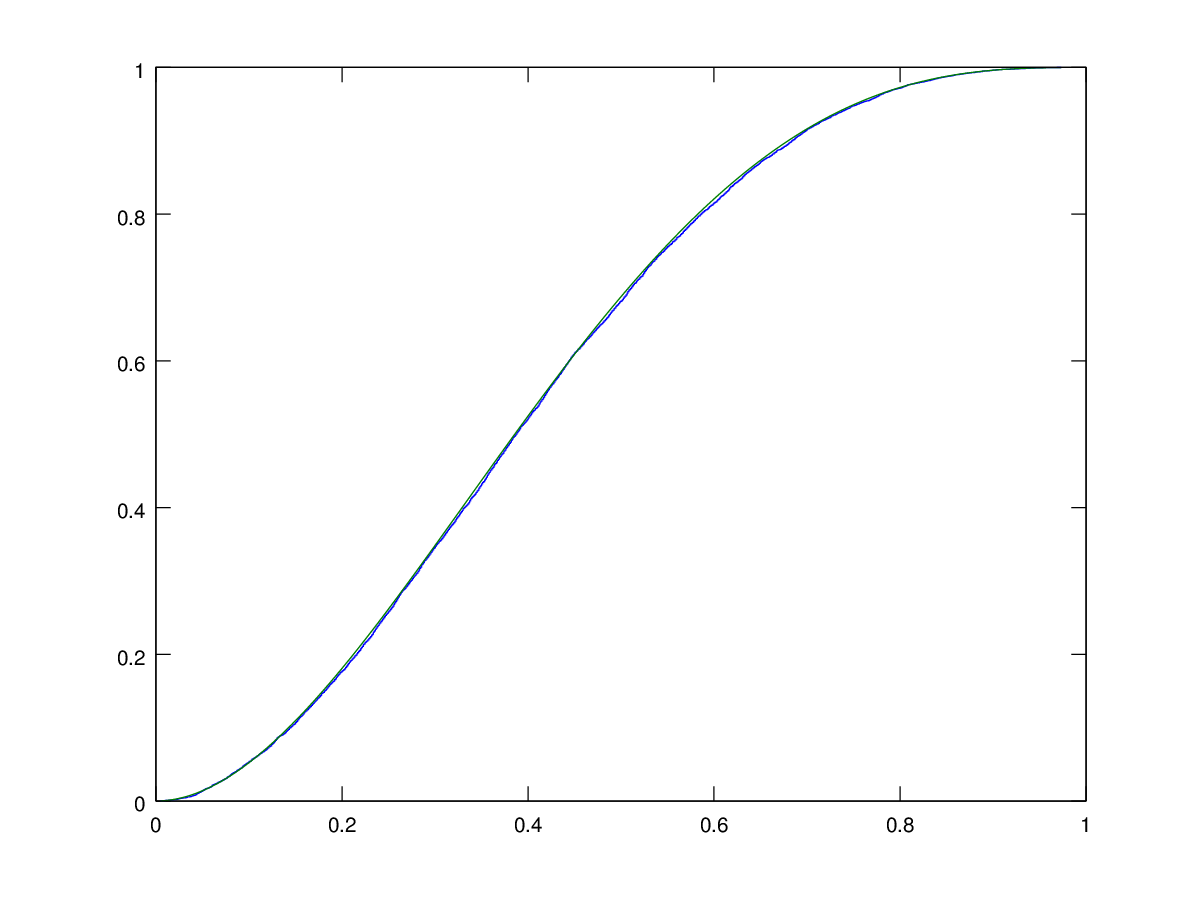
\includegraphics[width=8cm]{tarea3/problema3_4/poylaBeta.PNG}\pn
    Gr\'afica del histagrama de los radios ``finales'' de \texttt{10000} iteraciones del proceso 
	de urnas de P\'oyla (azul). En contraste con una distribución Beta (verde).\pn
\end{center}

En clase se demostró que los radios esperados tenían distribución Beta con los parámetros 
ya mencionados. En la gráfica se puede apreciar el parecido del resultado experimental con el teórico.\pn

P.S. \texttt{tic}, \texttt{toc} son funciones de octave para medir el tiempo de ejecución. En este caso
la ejecución duró cerca de un minuto. Lo cual era de esperarse, se realizaron poco más de \texttt{120,000,000} operaciones
y además, construir un gráfico con una retícula de \texttt{10000} puntos también es un proceso computacionalmente caro.